\documentclass[12pt]{article}
\usepackage[utf8]{inputenc}
\usepackage[margin=1in]{geometry}
\usepackage[spanish]{babel}\decimalpoint
\usepackage{setspace}\onehalfspacing
\usepackage{parskip} % Espacio entre parrafos.
\usepackage{graphicx} % Para usar comando \includegraphics[]{}
\usepackage{amssymb} % Para usar el simbolo del conj. de los Reales.
\usepackage{amsmath} % Para usar columnas vectoriales.
\usepackage{multirow} % Para unir multiples filas en una tabla.
\usepackage{hyperref} % Siempre debe ser el ultimo paquete.


\setcounter{tocdepth}{2} % Que no incluya subsubsections en la tabla de contenidos (toc).

%================================

\title{Clase 27. Integración y Sustitución Trigonométrica.}
\author{MIT 18.01: Single Variable Calculus.}
\date{}


\begin{document}

\maketitle


\begin{abstract}
\noindent Desde esta clase comenzamos a revisar \textbf{técnicas de integración} más avanzadas. En esta ocasión, nos centramos en integrar funciones trigonométricas usando sus identidades e introduciremos un método llamado sustitución trigonométrica.
\end{abstract}


\section{Identidades Trigonométricas (resumen).}

A partir del círculo unitario:

\begin{figure}[hbt!]
\centering
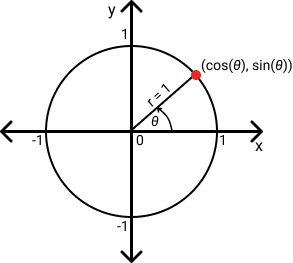
\includegraphics[scale=0.6]{img/trig-unit-circle.jpg}
\end{figure}

es posible encontrar las siguientes \textbf{identidades trigonométricas}:
\begin{align*}
&(1) \ \sin^{2}(\theta) + \cos^{2}(\theta) = 1 \\
&(2) \ \cos(2\theta) = \cos^{2}(\theta) - \sin^{2}(\theta); \quad \sin(2\theta) = 2\sin(\theta)\cos(\theta) \\
&(3) \ \cos^{2}(\theta) = \frac{1 + \cos(2\theta)}{2}; \quad \sin^{2}(\theta) = \frac{1 - \cos(2\theta)}{2}
\end{align*}
donde (1) es la identidad pitagórica, mientras que (2) y (3) son las fórmulas para el ángulo doble y para reducir/eliminar potencias de funciones trigonométricas\footnote{También permite obtener la fórmula del semiángulo.}, respectivamente.

Para esta clase, también vale la pena recordar las integrales indefinidas para el $\sin(x)$ y el $\cos(x)$.
\[
  \int \sin(x)dx = -\cos(x) + C \qquad \int \cos(x)dx = \sin(x) + C
\]
donde $C =$ constante.


\section{Integral del producto de potencias de seno y coseno.}

La integral que intentaremos evaluar a continuación, es la siguiente:
\[
  \int \sin^{n}(x)\cos^{m}(x)dx
\]
para $n \geq 0$ y $m \geq 0$ tal que $n, \ m \in \mathbb{Z}$.

\subsection{Al menos un exponente es impar.}

Cuando $n$ y/o $m$ son un número impar, la estrategia sugerida es factorizar la función trigonométrica tal que una (o ambas) quede con \textbf{exponente cuadrado}. La idea es, después, usar una de las \textbf{consecuencias de la identidad pitagórica}:
\[
  \sin^{2}(x) = 1 - \cos^{2}(x) \qquad \cos^{2}(x) = 1 - \sin^{2}(x)
\]

\textbf{Ejemplo 1.} Calcule la integral $\int \sin^{3}(x)\cos^{2}(x) dx$.

\textbf{Solución.} Como el $\sin^{3}(x)$ es de exponente impar, podemos establecer que $\sin^{3}(x) = \sin(x) \cdot \sin^{2}(x)$ y reescribir la integral de la siguiente manera:
\[
  \int \sin^{3}(x)\cos^{2}(x) dx = \int \left(\sin(x)\sin^{2}(x)\right)\cos^{2}(x) dx
\]
Hemos factorizado al $\sin^{3}(x)$ de esa manera, porque podemos reemplazar al $\sin^{2}(x)$ con la consecuencia de la identidad pitagórica para aquella función.
\[
 \int \sin^{3}(x)\cos^{2}(x) dx = \int \left(\sin(x)[1 - \cos^{2}(x)]\right)\cos^{2}(x) dx
\]
Luego, usemos el método de sustitución estableciendo que $u = \cos(x)$. Esto implica que el diferencial $du = -\sin(x)dx$ y que:

\[
  \int \sin^{3}(x)\cos^{2}(x) dx = \int -(1 - u^{2}) u^{2}du
                                 = - \int (u^{2} - u^{4})du
                                 = - \left(\frac{u^{3}}{3} - \frac{u^{5}}{5}\right) + C
\]
Reemplazando a $u = \cos(x)$ en la antiderivada de arriba obtenemos la respuesta de este ejemplo.
\[
  \int \sin^{3}(x)\cos^{2}(x) dx = \frac{\cos^{5}(x)}{5} - \frac{\cos^{3}(x)}{3} + C
\]

\subsection{Ambos exponentes son pares.}

Cuando tanto $n$ como $m$ son números pares, la mejor estrategia es partir usando la \textbf{fórmula para reducir/eliminar exponentes} del $\sin(x)$ y del $\cos(x)$.

\textbf{Ejemplo 2.} Calcule la antiderivada de $\int \sin^{2}(x)\cos^{2}(x) dx$.

\textbf{Solución.} Como los exponentes del $\sin(x)$ y del $\cos(x)$ son números pares, podemos comenzar simplificar la integral usando la fórmula de reducción de exponentes.
\begin{align*}
  \int \sin^{2}(x)\cos^{2}(x) dx &= \int \left(\frac{1 - \cos(2x)}{2} \cdot \frac{1 + \cos(2x)}{2}\right) dx \\
                                 &= \int \left(\frac{1 - \cos^{2}(2x)}{4}\right) dx \\
  \int \sin^{2}(x)\cos^{2}(x) dx &= \frac{1}{4} \cdot \int (1 - \cos^{2}(2x)) dx
\end{align*}
Aún quedamos con el $\cos(x)$ con exponente par, por lo que podemos usar otra vez la fórmula de reducción de exponentes, pero teniendo en consideración que ahora $x = 2x$.
\begin{align*}
  \int \sin^{2}(x)\cos^{2}(x) dx &= \frac{1}{4} \cdot \int \left(1 - \frac{1 + \cos(2(2x))}{2}\right) dx \\
                                 &= \frac{1}{4} \cdot \int \left(\frac{1 + \cos(4x)}{2}\right) dx \\
  \int \sin^{2}(x)\cos^{2}(x) dx &= \frac{1}{8} \cdot \int (1 + \cos(4x)) dx
\end{align*}
Finalmente, para calcular la antiderivada podemos usar el método de sustitución, definiendo que $u = 4x$ y que $du = 4dx$ como consecuencia de aquello.
\[
\int \sin^{2}(x)\cos^{2}(x) dx = \frac{1}{8} \cdot \int \frac{1}{4} \cdot (1 + \cos(u)) du
                               = \frac{1}{32} (u - \sin(u)) + C
\]
Reemplazando $u = 4x$ en la antiderivada, obtenemos que:
\[
  \int \sin^{2}(x)\cos^{2}(x) dx = \frac{4x}{32} - \frac{\sin(4x)}{32} + C = \frac{x}{8} - \frac{\sin(4x)}{32} + C
\]

\section{Sustitución Trigonométrica.}

Cuando buscamos resolver integrales con un integrando del tipo $\sqrt{a + x^{2}}$ o similares, con $a$ siendo una constante, es más eficiente reemplazar la variable de integración por una \textbf{función trigonométrica}. Este proceso se conoce como \textbf{Sustitución Trigonométrica}.

La sustitución trigonométrica es similar al método de sustitución que hemos estudiado antes: Reemplazamos la variable de integración, resolvemos la integral y, posteriormente, restituímos la variable original. Se diferencia en que el cambio se hace con una función nueva, que en este caso es trigonométrica.

Antes, cuando aplicábamos el método de sustitución, reemplazábamos la variable de integración por otra que estaba en función de ella. Por ejemplo, establecíamos que $u = x^{2}$, donde $u = u(x)$. Ahora señalaremos, por ejemplo, que $x = a\sin(\theta)$. Es decir, la variable de integración será una nueva función, usando una de las trigonométricas.

Al sustituir la variable de integración, la idea después es volver a ella. En ocasiones, cuando lo hacemos con funciones trigonométricas, la variable de estas últimas también debemos retornarla a su forma original, lo cual es posible con sus \textbf{inversas}. Ahí, el proceso recibe el nombre de \textbf{Sustitución Trigonométrica Inversa}.

%Si reemplazamos la variable de integración, la idea después es volver a ella y aquello es posible con las funciones trigonométricas usando sus \textbf{inversas}\footnote{Teniendo en cuenta la restricción correspondiente a sus dominios.}. Es por ello que esta técnica también recibe el nombre de \textbf{Sustitución Trigonométrica Inversa}.

\textbf{Ejemplo 3.} Calcule el área de altura $b$ del siguiente círculo de radio $r = a$.

\begin{figure}[hbt!]
\centering
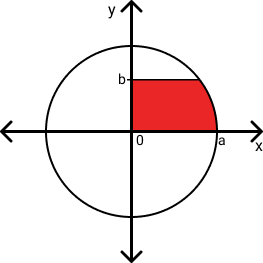
\includegraphics[scale=0.6]{img/trig-int-example-1.jpg}
\end{figure}

\textbf{Solución.} Debido a que una parte del área es curvada (el arco del círculo), podemos optar por calcularla a partir de la suma de las áreas de rectángulos infinitamente delgados. La decisión que debemos tomar es si éstos serán verticales u horizontales.

Si usamos rectángulos verticales, o en función de $x$, tendremos que lidiar con el problema de calcular el área para dos funciones: una para $y = b$ y otra para el arco del círculo. Sin embargo, esto no ocurre si lo hacemos en función de $y$ (i.e, rectángulos horizontales), ya que solo tomará el valor del arco.

El valor del arco del círculo, está dado por la ecuación de esta figura, la que corresponde a:
\[
  a^{2} = x^{2} + y^{2}
\]
Vamos a trabajar en función de $y$, por lo tanto debemos reordenar la ecuación de arriba despejando a $x$:
\[
  x(y) = \sqrt{a^{2} - y^{2}}
\]
La integral, que denotaremos como $A$, la calcularemos a partir de $x(y)$, de manera que la suma acumulada la haremos entre $0 \leq y \leq b$.
\[
  A = \int_{0}^{b} \left(\sqrt{a^{2} - y^{2}}\right) dy
\]
Como tenemos una raíz cuadrada con una expresión algebraica en su interior, la mejor opción es hacer una \textbf{sustitución trigonométrica}. Para esto, usaremos \textbf{coordenadas polares}.

De forma resumida, el \textbf{sistema de coordenadas polares} es aquel que especifica la ubicación de un punto en un plano por medio de una \textbf{distancia y dirección}. En la siguiente imagen podemos ver una representación de este tipo de sistema de coordenadas.

\begin{figure}[hbt!]
\centering
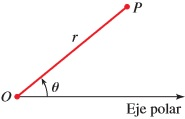
\includegraphics[scale=0.95]{img/polar-coord-1.jpg}
\caption{(Steward, et.al; 2017: 542)}
\end{figure}

El centro $O$ se llama \textbf{polo} y el rayo, \textbf{eje polar}. La \textbf{distancia} es el largo de este último, denotado en la imagen como $r$. Para conocer al punto $P$, se traza un segmento $OP$ también de longitud $r$ y, entre éste y el rayo, se forma un ángulo $\theta$, que nos da la \textbf{dirección}. Así, la posición de $P$ en el \textbf{sistema de coordenadas polares} es el par ordenado $P(r, \ \theta)$.

Si la coordenada polar del punto $P(r, \ \theta)$ la ubicamos en el primer cuadrante de un sistema de coordenadas rectangulares (el que usamos habitualmente), podemos dibujar un triángulo rectángulo como el que vemos a continuación.

\begin{figure}[hbt!]
\centering
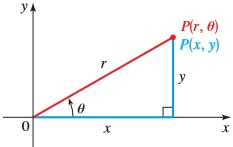
\includegraphics[scale=0.95]{img/polar-coord-2.jpg}
\caption{(Steward, et.al; 2017: 543)}
\end{figure}

Los valores de los lados $x$ e $y$ del triángulo rectángulo podemos conocerlos a partir del $\cos(\theta)$ y el $\sen(\theta)$ como:
\[
  x = r \cdot \cos(\theta) \qquad y = r \cdot \sin(\theta)
\]
La hipotenusa del triángulo rectángulo está dada por la distancia $r$ de la coordenada polar de $P(r, \theta)$ y como coincide con estar con un mismo punto $P(x, \ y)$ del sistema rectangular, podemos generalizarlo como:
\[
  P(r, \ \theta) = P(x, \ y) = P(r \cdot \cos(\theta), \ r \cdot \sin(\theta))
\]
Ahora usemos esta última idea para resolver el Ejemplo 2.

Adentro del área que buscamos calcular del circulo, podemos ubicar un punto en coordenadas polares, donde la distancia está dada por el radio $r = a$ y de dirección $\theta_{0}$.

\begin{figure}[hbt!]
\centering
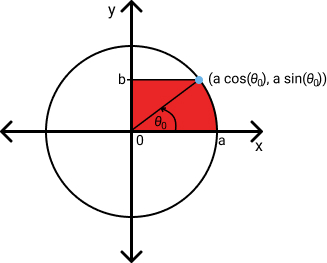
\includegraphics[scale=0.7]{img/trig-int-example-2.jpg}
\end{figure}

Recordemos que $x(y) = \sqrt{a^{2} - y^{2}}$ y, usando coordenadas polares, debería cumplirse que también es igual a $a \cdot \cos(\theta_{0})$ sabiendo que $y = a \cdot \sin(\theta_{0})$.
\[
  x(a \cdot \sin(\theta_{0})) = \sqrt{a^{2} - (a \cdot \sin(\theta_{0})^{2}}
                              = a \cdot \sqrt{1 - \sin^{2}(\theta_{0})}
                              = a \cdot \sqrt{\cos^{2}(\theta_{0})}
                              = a \cdot \cos(\theta_{0})
\]
Por lo tanto, realicemos la \textbf{sustitución trigonométrica} estableciendo que $y = a \cdot \sin(\theta_{0})$ y, en consecuencia, que $dy = a \cdot \cos(\theta_{0}) d\theta_{0}$. La trabajaremos primero como una antiderivada.
\[
  \int \left(\sqrt{a^{2} - y^{2}}\right) dy = \int (a \cdot \cos(\theta_{0})) \cdot (a \cdot \cos(\theta_{0}) d\theta_{0}
                                            = \int a^{2} \cdot \cos^{2}(\theta_{0}) d\theta_{0}
                                            = a^{2} \int \cos^{2}(\theta_{0}) d\theta_{0}
\]
Como el la función coseno es de exponente par, podemos usar la fórmula trigonométrica para reducirlo.
\begin{align*}
  \int \left(\sqrt{a^{2} - y^{2}}\right) dy &= a^{2} \cdot \int \frac{1 + \cos(2\theta_{0})}{2} d\theta_{0} \\
                                            &= \frac{a^{2}}{2} \cdot \left(\theta_{0} + \frac{\sin(2\theta_{0})}{2}\right) + C \\
                                            &= a^{2} \cdot \left(\frac{\theta_{0}}{2} + \frac{\sin(2\theta_{0})}{4}\right) + C
\end{align*}
Ahora, llevemos de vuelta esta integral indefinida a sus variables iniciales.

Lo primero es trabajar solo con $\theta_{0}$. Como vemos en la antiderivada de arriba, tenemos el $\sin(2\theta_{0})$, de manera que podemos usar la fórmula del ángulo doble para quitar ese $2$ de la función seno.
\[
  \int \left(\sqrt{a^{2} - y^{2}}\right) dy = a^{2} \cdot
                                              \left(\frac{\theta_{0}}{2} + \frac{2\sin(\theta_{0})\cos(\theta_{0})}{4}\right) + C
                                            = a^{2} \cdot
                                              \left(\frac{\theta_{0}}{2} + \frac{\sin(\theta_{0})\cos(\theta_{0})}{2}\right) + C
\]
Además, previamente establecimos que $y = a \cdot \sin(\theta_{0})$. Al despejar a la función seno, obtenemos que:
\[
  \sin(\theta_{0}) = \frac{y}{a}
\]
Y para conocer a $\theta_{0}$ solo necesitamos calcular el arcoseno o $\sin^{-1}(\cdot)$.
\[
  \theta_{0} = \sin^{-1}\left(\frac{y}{a}\right)
\]
Por lo tanto, podemos reemplazar aquello en la ecuación de la integral:
\[
\int \left(\sqrt{a^{2} - y^{2}}\right) dy = a^{2} \cdot
                                            \left(\frac{\sin^{-1}(y/a)}{2} + \frac{\sin(\theta_{0})\cos(\theta_{0})}{2}\right) + C
\]
Es posible deducir que el $\cos(\theta_{0}) = x/a$. Ya conocemos el $\sin(\theta_{0})$, por lo tanto ambas podemos incorporarlas a la integral:
\begin{align*}
\int \left(\sqrt{a^{2} - y^{2}}\right) dy &= a^{2} \cdot
                                            \left(
                                              \frac{\sin^{-1}(y/a)}{2} + \left[\frac{1}{2} \cdot \frac{y}{a} \cdot \frac{x}{a}\right]
                                            \right)
                                            + C \\
                                          &= \frac{a^{2}\sin^{-1}(y/a)}{2} +
                                            a^{2} \cdot \left[\frac{1}{2} \cdot \frac{y}{a} \cdot \frac{x}{a}\right] + C \\
                                          &= \frac{a^{2}\sin^{-1}(y/a)}{2} + \frac{1}{2} \cdot y \cdot x + C
\end{align*}
No olvidemos que $x(y) = \sqrt{a^{2} - y^{2}}$.
\[
  \int \left(\sqrt{a^{2} - y^{2}}\right) dy = \frac{a^{2}\sin^{-1}(y/a)}{2} + \frac{y \cdot \sqrt{a^{2} - y^{2}}}{2} + C
\]
Finalmente, busquemos el área $A$ delimitando a la integral de arriba en $y = 0$ e $y = b$.
\[
  A = \int_{0}^{b} \left(\sqrt{a^{2} - y^{2}}\right) dy
    = \left[\frac{a^{2}\sin^{-1}(y/a)}{2} + \frac{y \cdot \sqrt{a^{2} - y^{2}}}{2}\right]_{0}^{b}
    = \frac{a^{2}\sin^{-1}(b/a)}{2} + \frac{b \cdot \sqrt{a^{2} - b^{2}}}{2}
\]
Veamos que esta área $A$ es la suma de las dos partes en que se divide al trazar la distancia del punto $(a \cdot \cos(\theta_{0}), a \cdot \sin(\theta_{0}))$, las que corresponden al sector circular y el triángulo.

\end{document}
